\documentclass[11pt,a4paper]{article}

% Essential packages
\usepackage[utf8]{inputenc}
\usepackage[T1]{fontenc}
\usepackage{amsmath,amsthm,amssymb}
\usepackage{hyperref}
\usepackage{cleveref}
\usepackage{tikz}
\usetikzlibrary{arrows.meta,positioning,shapes.geometric}

% Theorem environments
\newtheorem{theorem}{Theorem}[section]
\newtheorem{lemma}[theorem]{Lemma}
\newtheorem{proposition}[theorem]{Proposition}
\newtheorem{corollary}[theorem]{Corollary}
\theoremstyle{definition}
\newtheorem{definition}[theorem]{Definition}
\newtheorem{example}[theorem]{Example}
\theoremstyle{remark}
\newtheorem{remark}[theorem]{Remark}

% Open question environment
\newenvironment{openquestion}{\par\textbf{Open Question.}\itshape}{\par}

\title{Notes Toward an Iterative AI-Assisted Writing and Study Process}
\author{AI Notes}
\date{\today}

\begin{document}

\maketitle

\begin{abstract}
This note records a tentative workflow in which a language model assists the drafting of a technical document while a human author performs systematic verification. The central claim is not that the model is a reliable authority, but that repeated drafting, checking, and revision can support a study process that is closer in spirit to conventional literature search and verification, while lowering the cost of producing and updating written drafts. The note aims to be conservative: where a claim is not justified by reasoning or cited sources, it is stated as an open question.
\end{abstract}

\section{Introduction}
\label{sec:introduction}

In many technical domains, writing and studying are intertwined. Before modern generative tools, large revisions to a draft were often expensive, which encouraged a separation between a prolonged study phase and a later writing phase. The present note outlines a workflow in which draft production is cheap enough that study and writing can proceed in shorter cycles, with the intent that each cycle improves both the document and the author’s understanding.

The note assumes only the familiar backbone of scholarly work: search for credible sources, attempt to understand them, and verify conclusions against definitions, known results, and proofs. The proposed change is primarily one of tooling and iteration cadence; see \cref{sec:loop,sec:checklist}.

\section{Background and motivation}
\label{sec:background}

Contemporary large language models are trained on broad corpora and frequently exhibit what appears to be ``common-sense'' competence across many domains. This observation is widely discussed under the umbrella of ``foundation models'' \cite[Section~1]{Bommasani2021}. At the same time, there is substantial evidence that language models can produce fluent but false or misleading outputs, motivating explicit evaluation of truthfulness and verification practices \cite[Section~1]{Lin2021TruthfulQA}.

This note adopts a cautious stance: model outputs are treated as \emph{draft hypotheses} rather than authoritative statements. The workflow’s purpose is to exploit the speed of draft generation while maintaining epistemic discipline through explicit verification steps.

\section{The iterative writing-and-study loop}
\label{sec:loop}

The workflow is described as a sequence of stages that repeat over versions of a document.

\subsection{High-level stages}
\label{sec:stages}

\begin{enumerate}
  \item \textbf{Draft generation from a topic seed.} A model produces a draft that attempts to explain a topic, including definitions, claims, and references where possible.

  \item \textbf{Human review for clarity and plausibility.} The human reader flags unclear passages, missing definitions, suspicious steps in arguments, and claims that appear too strong relative to the evidence provided.

  \item \textbf{Verification and reference checking.} For each nontrivial claim, the human attempts to locate an authoritative source (textbook, lecture notes, or peer-reviewed literature) or to supply a proof. Claims without adequate support are either removed, weakened, or explicitly marked as open questions; see \cref{sec:open-questions}.

  \item \textbf{Revision and consolidation.} The draft is revised to incorporate corrections, tightened statements, and improved structure. The bibliography and internal cross-references are updated so that later reviews can target specific items precisely.

  \item \textbf{Iteration and versioning.} The process repeats. Each iteration yields a new version of the document, ideally with fewer unsupported claims and clearer dependencies between statements.
\end{enumerate}

\subsection{Rationale and intended outcomes}
\label{sec:rationale}

The following points motivate the loop above:

\begin{enumerate}
  \item Models often produce coherent cross-domain prose and can propose candidate structures for an unfamiliar topic. This can reduce the initial cost of outlining a document and enumerating terms to define.

  \item Repeated drafting under a fixed topic can help surface connections between subtopics. In favorable cases, successive drafts refine the conceptual graph by making dependencies explicit.

  \item A human reviewer can use the draft as a checklist of questions: which definitions are missing, which steps require justification, and which references actually support the claims stated.

  \item Each generation--review cycle yields a new version of the document that can be compared against previous versions and against a fixed set of verification expectations; see \cref{sec:checklist}.

  \item Over iterations, the document may converge toward a state in which most claims are grounded in cited sources or proved arguments. Unresolved items are collected as open questions, potentially indicating directions for further study; see \cref{sec:open-questions}.

  \item The underlying scholarly backbone---search, study, and verification---is unchanged. The proposed workflow merely replaces some drafting labor with model-assisted drafting while retaining human responsibility for verification.

  \item Lower writing cost blurs the boundary between studying and writing: when revisions are cheap, a draft can evolve more like a software artifact, where refactoring and frequent updates are routine rather than exceptional.

  \item One may view the process as ``verification-driven composing,'' loosely analogous to test-driven development: informal expectations guide review, and the document’s evolution can be compared against those expectations. As in software testing, the expectations themselves may be wrong and may need revision.
\end{enumerate}

\section{Diagram of the loop}
\label{sec:diagram}

\begin{figure}[ht]
\centering
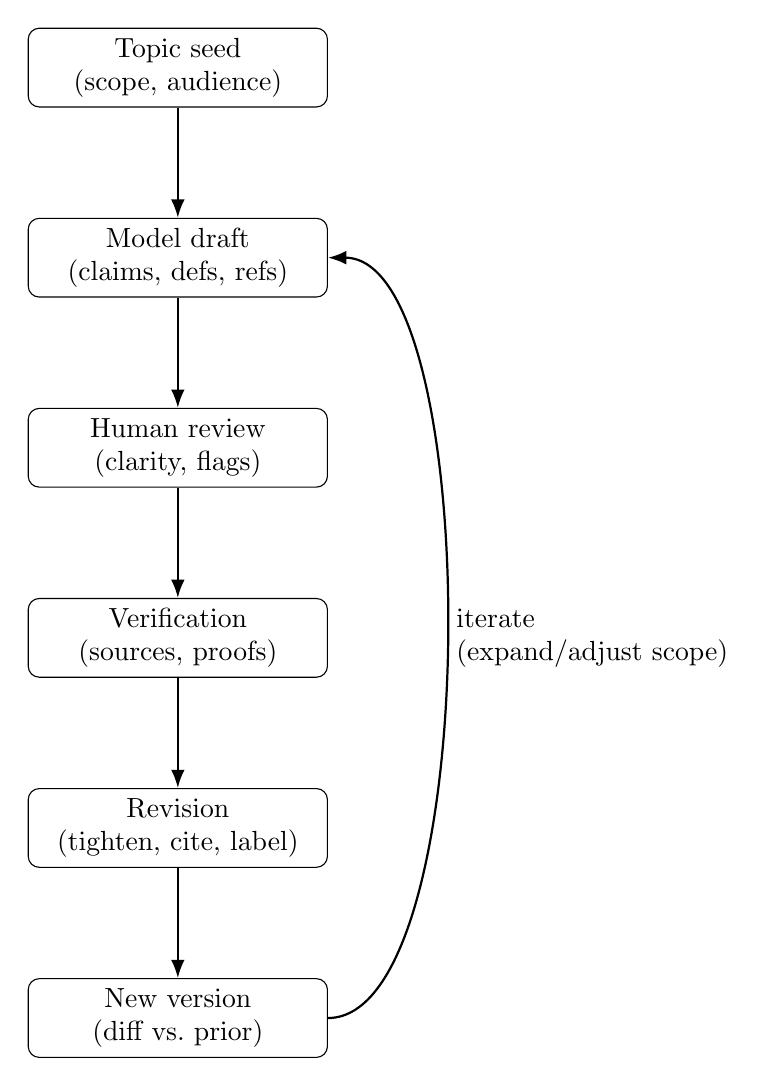
\begin{tikzpicture}[
  node distance=14mm,
  box/.style={draw, rounded corners, align=center, minimum width=38mm, minimum height=10mm},
  arrow/.style={-Latex, thick}
]
  \node[box] (seed) {Topic seed\\(scope, audience)};
  \node[box, below=of seed] (draft) {Model draft\\(claims, defs, refs)};
  \node[box, below=of draft] (review) {Human review\\(clarity, flags)};
  \node[box, below=of review] (verify) {Verification\\(sources, proofs)};
  \node[box, below=of verify] (revise) {Revision\\(tighten, cite, label)};
  \node[box, below=of revise] (version) {New version\\(diff vs.\ prior)};

  \draw[arrow] (seed) -- (draft);
  \draw[arrow] (draft) -- (review);
  \draw[arrow] (review) -- (verify);
  \draw[arrow] (verify) -- (revise);
  \draw[arrow] (revise) -- (version);
  \draw[arrow] (version.east) .. controls +(20mm,0) and +(20mm,0) .. node[right,align=left]{iterate\\(expand/adjust scope)} (draft.east);
\end{tikzpicture}
\caption{A draft generation--review--verification loop. The model contributes text and candidate structure; the human retains responsibility for verification and for deciding which claims to keep.}
\label{fig:loop}
\end{figure}

As illustrated in \cref{fig:loop}, the loop emphasizes explicit verification as a distinct stage rather than an implicit afterthought.

\section{Practical review checklist}
\label{sec:checklist}

This section records a lightweight checklist intended for repeated use during revisions. It is aligned with the repository’s agent review expectations and is meant to be applied both by humans and by agents acting in a reviewer role.

\begin{enumerate}
  \item \textbf{Academic style.} Is the tone formal and precise? Are terms defined before use? Is the structure appropriate (abstract, sections, conclusion)?

  \item \textbf{Correctness discipline.} Are all substantive claims either proved, justified by reasoning, or supported by a cited source? If not, are they weakened or moved to \cref{sec:open-questions}?

  \item \textbf{Citation precision.} For each external claim, is there a Bib\TeX{} entry and a pinpoint citation (at least to a section, and to a page when quoting or relying on a specific passage)?

  \item \textbf{Cross-references.} Are internal references provided via \texttt{\textbackslash label} and \texttt{\textbackslash cref} for key sections, figures, and equations?

  \item \textbf{Version deltas.} Relative to the previous version, what changed and why? Which open questions were resolved, and which new ones were introduced?
\end{enumerate}

\section{Limitations and open questions}
\label{sec:open-questions}

The proposed workflow is intentionally conservative about what it guarantees.

\begin{openquestion}
Under what conditions (topic difficulty, available sources, reviewer expertise) does the loop in \cref{sec:loop} reliably converge toward a document with mostly verified claims, rather than stabilizing on plausible but incorrect narratives?
\end{openquestion}

\begin{openquestion}
What review practices most effectively detect ``plausible fallacies'' in model-generated text, beyond standard citation checking (e.g., formal proof reconstruction, independent derivations, or adversarial spot checks)?
\end{openquestion}

\begin{openquestion}
How should one quantify progress across iterations (e.g., number of unsupported claims, proportion of statements with proofs/citations, or reviewer confidence), and how well do such metrics correlate with actual correctness?
\end{openquestion}

\section{Conclusion}
\label{sec:conclusion}

This note proposes an iterative workflow that treats model outputs as drafts to be verified. The intent is to preserve the standard scholarly backbone of search, study, and verification while lowering the mechanical cost of drafting and revision. The workflow’s value depends on rigorous review practices, precise citations, and a willingness to mark unresolved points explicitly as open questions.

\bibliographystyle{plain}
\bibliography{references}

\end{document}

